\section{Group Extension \& Local Headline} % (fold)
\label{sec:group_extension_local_headline}

\subsection{Group Extension} % (fold)
\label{sub:group_extension}

We consider that {\tt Social News} has been deployed on top of the social network depicted in
figure~\ref{fig:sn-news-init}. Nodes $\nu_8$, $\nu_4$ and $\nu_2$ in the figure (green colored) submit news concurrently.
Let $\nu_8^S=<\alpha_0^8,\ldots,\alpha_\jmath^8>$, $\nu_4^S=<\alpha_0^4,\ldots,\alpha_\ell^4>$ and
$\nu_2^S=<\alpha_0^2,\ldots,\alpha_\imath^2>$ denote the messages sent out by $\nu_8$, $\nu_4$ and $\nu_2$, respectively.
Here, we study the group extension initiated by $\nu_8$. As well, we discuss the peculiarities of a possible group
extension between $\nu_2$ and $\nu_4$.

Let $g^{\nu_8}$ denote the group initiated by $\nu_8$ to pass his headlines and let $P_{g^{\nu_8}}$ denote the process
representing this group extension. Initially, since $\nu_8$ only has a direct link to $\nu_6$ and $\nu_{10}$, the
extension will start with the possible behaviors at these three nodes. Let $P^{\nu_8}$, $P^{\nu_6}$ and $P^{\nu_{10}}$
denote the processes corresponding to the behaviors of nodes $\nu_8$, $\nu_6$ and $\nu_{10}$, respectively. For the
communication with future members of $g^{\nu_8}$, we allow $\nu_8$ to create a group of channels, say $G_8$. Each member
of the group will use a different instance of this channel group.

We assume that the connection between $\nu_8$ and $\nu_6$ is materialized by the name $a$, while the connection between
$\nu_8$ and $\nu_{10}$ is materialized by the name $b$. Since these names ensued from the initial structure of the social
network, we cannot consider them as secure enough for communication during the group extension. Nevertheless, they will
be used to communicate the new channels for the extension. In order to prevent any information breach (e.g., $\nu_6$
accessing any information exclusively destined for $\nu_{10}$, and vice versa), we assume that elementary news do not
travel directly through the channels. Rather, a set of news is represented following a certain format before it is sent
through a channel. These formats can be regarded as object representations of the news being submitted. Note that we do
not assume that all the news being submitted are the same type. Let $T_0^8,\ldots,T_\jmath^8$ denote the types of the
news submitted by $\nu_8$. Each of the formats is a special composition of the elementary news types
$T_0^8,\ldots,T_\jmath^8$. We introduce these composition types as the channel types for instances of $G_8$. Let
$\mathbf{C}_{\nu_6^8}<T_0^8,\ldots,T_\jmath^8>$ denote the type of the package $\nu_8$ will exclusively send to $\nu_6$.
For sake of simplicity, we adopt $\mathbf{C}_{\nu_6^8}$. Similarly, let $\mathbf{C}_{\nu_{10}^8}$ denote the type of the
package $\nu_8$ sends to $\nu_{10}$. Although all these types are structurally equivalent, we assume that they can only
be interpreted by a node prepared to read from/write to them. Following these new types we shall create special channels
for appropriate communication in $g^{\nu_8}$. Figure~\ref{fig:sn-news-v8-channels} depicts the creation of such instance
channels.

\begin{figure}
	\centering 
	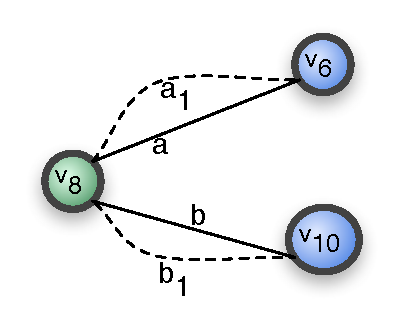
\includegraphics[width=.35\textwidth]{social_news-piv8} 
	\caption{Public and Secret Communication Channels} 
	\label{fig:sn-news-v8-channels} 
\end{figure}

From the description in section~\ref{sec:application}, we extracted a protocol corresponding to the group extension.
Figure~\ref{fig:subgextprot} depicts the sequence diagram corresponding to this protocol.
\begin{figure}
	\centering 
	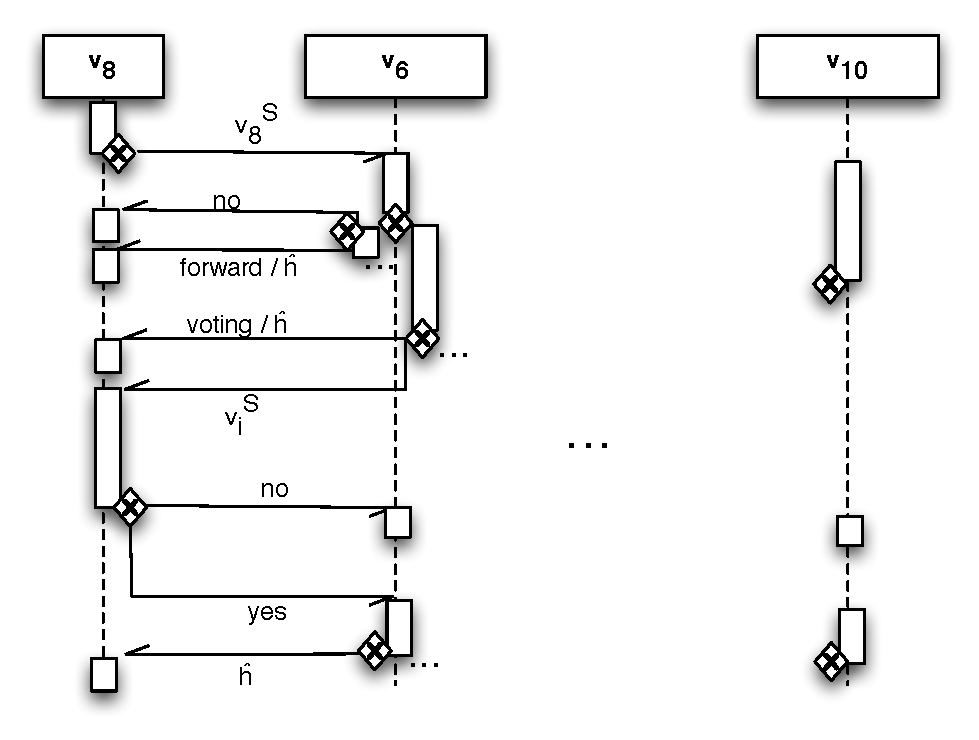
\includegraphics[width=.7\textwidth]{social_news-gext-prot} 
	\caption{group extension protocol in {\tt Social News} - $g^{\nu_8}$'s case} 
	\label{fig:subgextprot} 
\end{figure}

Equation~\ref{eq:gv8-formation} represents our specification of $g^{\nu_8}$'s formation.
\begin{equation}
	\label{eq:gv8-formation}
	\boxed{P_{g^{\nu_8}}\overset{df}{=}(\nu G_8)(P^{\nu_8}\mid P^{\nu_6} \mid P^{\nu_{10}})}
\end{equation}

Since a group formation is not mandatory at this stage, $P^{\nu_8}$ can decide to do nothing, send the message
($\nu_8^S$) to both\footnote{The reader should note that because we are using an asynchronous $\pi-calculus$ and that
members can act both as source and sink, we cannot afford to share the same channel between more than two members.}
$\nu_6$ and $\nu_{10}$ (process $P^{\prime\nu_8}$), or send it to $\nu_6$ only (process $P^{\prime\prime\nu_8}$) or
$\nu_{10}$ only (process $P^{\prime\prime\prime\nu_8}$). After sending the message, the rest of $P^{\nu_8}$'s behavior
depends on the branch it has chosen: $P^{\nu_8}_{\propto a_1R}$ and/or $P^{\nu_8}_{\propto b_1R}$. Both processes are
similar, the only difference being the channel used for communication.

\begin{equation} 
	\label{eq:pv8expr}
	\begin{gathered}
		P^{\nu_8} \overset{df}{=} \mathbf{0} + (\nu a_1:G_8[\mathbf{C}_{\nu_6^8}], \nu b_1:G_8[\mathbf{C}_{\nu_{10}^8}])(P^{\prime\nu_8} + (P^{\prime\prime\nu_8} + P^{\prime\prime\prime\nu_8}))\\
		P^{\prime\nu_8}\overset{df}{=}P^{\prime\prime\nu_8}\mid P^{\prime\prime\prime\nu_8}\\
		P^{\prime\prime\nu_8}\overset{df}{=}\overset{-}{a}<a_1>.\overset{-}{a}_1<\nu_8^S>.P^{\nu_8}_{\propto a_1R}	\\
		P^{\prime\prime\prime\nu_8}\overset{df}{=}\overset{-}{b}<b_1>.\overset{-}{b}_1<\nu_8^S>.P^{\nu_8}_{\propto b_1R}		
	\end{gathered}
\end{equation}

According to the protocol, invited neighbors are given two options: \emph{decline} or \emph{accept}. A strong declination
will be a ``{\tt no}'' message sent by an invited member, while a weak one corresponds to a ``{\tt forward}'' message.
When $\nu_8$ receives a ``{\tt forward}'' message, he also expects all the channels which have been created for
interaction between him and the decliner's neighbor(s). On the other hand, an invitation can be accepted, ``{\tt
voting}'' or another submission $\nu_\imath^S$ is sent as message. In the latter case, $\nu_8$ will decide whether to
accept the condition or not. Equation~\ref{eq:pv8expr6} specifies that phase.

\begin{equation}
	\label{eq:pv8expr6}
	\begin{gathered}
		P^{\nu_8}_{\propto a_1R}\overset{df}{=}((a_1(m^\lambda).(\overset{-}{m}^\lambda\mid (no.\tau.P^{\nu_8}_{\propto a_1} + forward.a_1(\hat{g})\mid !P^{\nu_8}_{\propto R} + \hat{g}.!P^{\nu_8}_{\propto R} +\\ voting.\tau.P^{\nu_8}_{\propto a_1} + \nu_\imath^S.(\overset{-}{a}_1<no> + \overset{-}{a}_1<yes>.\tau).P^{\nu_8}_{\propto a_1}))))\\
		P^{\nu_8}_{\propto b_1R}\overset{df}{=}((b_1(m^\lambda).(\overset{-}{m}^\lambda\mid (no.\tau.P^{\nu_8}_{\propto b_1} + forward.b_1(\hat{h})\mid !P^{\nu_8}_{\propto R} + \hat{h}.!P^{\nu_8}_{\propto R} +\\ voting.\tau.P^{\nu_8}_{\propto b_1} + \nu_\imath^S.(\overset{-}{b}_1<no> + \overset{-}{b}_1<yes>.\tau).P^{\nu_8}_{\propto b_1}))))\\
		P^{\nu_8}_{\propto R}\overset{df}{=}((r(m^\delta).(\overset{-}{m}^\delta\mid (no.\tau + forward.r(\hat{f})\mid !P^{\nu_8}_{\propto R} + \hat{f}.!P^{\nu_8}_{\propto R} + voting.\tau +\\ \nu_\jmath^S.(\overset{-}{r}<no> + \overset{-}{r}<yes>.\tau))))) (\mbox{ with } r\in\hat{g}\cup\hat{h})\\
	\end{gathered}
\end{equation}

At any time $\nu_8$ keeps listening to all the channels he created. New members might contact him on the new names he
received or other members might send him new names as the extension proceeds. When the group extension delay passes, he
then notifies members in voting state that the deadline has passed. He sends a common channel that all members should use
to vote. Equations~\ref{eq:pv8expr4} and~\ref{eq:pv8expr5} define this phase. We represent this as a non deterministic
choice between time-up and the continuous listening mode. Once the time-up notification (i.e., at least one member has
accepted the invitation) has been sent, $\nu_8$ gets ready for the voting procedure, which marks the end of the group
extension phase. Figure~\ref{fig:groupformv8} depicts the extension of group $g^{\nu_8}$.

\begin{figure}
	\centering 
	\subfloat[During group extension]{\label{fig:groupext-during}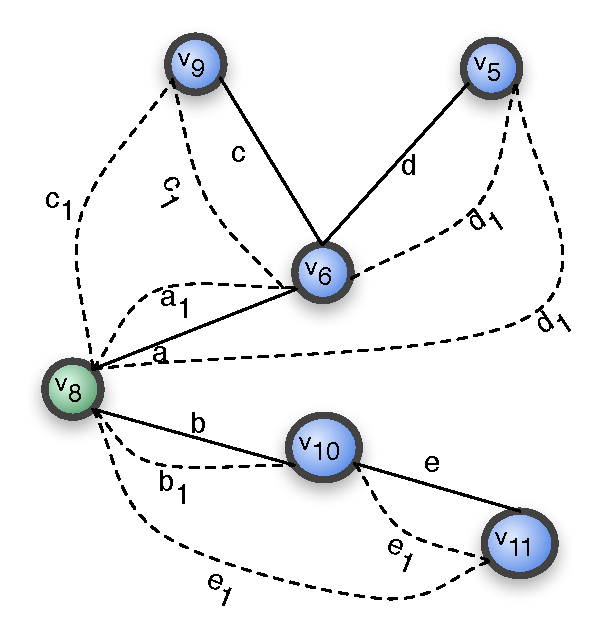
\includegraphics[width=0.35\textwidth]{social_news-gv8-dformation}} 
	\subfloat[After group extension]{\label{fig:groupext-done}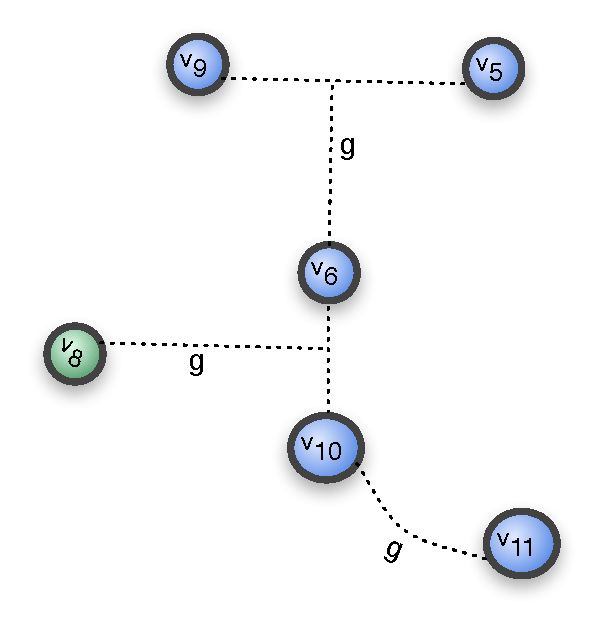
\includegraphics[width=0.35\textwidth]{social_news-gv8-aformation}}
	\caption{Extending group $g^{\nu_8}$} 
	\label{fig:groupformv8} 
\end{figure}

\begin{equation}
	\label{eq:pv8expr4}
	\begin{gathered}
	P^{\nu_8}_{\propto a_1}\overset{df}{=}(P^{\nu_8}_{TimeUp} + P^{\nu_8}_{\propto a_1R})\\
	P^{\nu_8}_{\propto b_1}\overset{df}{=}(P^{\nu_8}_{TimeUp} + P^{\nu_8}_{\propto b_1R})
	\end{gathered}
\end{equation}

\begin{equation}
	\label{eq:pv8expr5}
	\begin{gathered}
	P^{\nu_8}_{TimeUp}\overset{df}{=}(\nu g:G_8[\mathbf{C}_{\nu^8}])\overset{-}{s}<g>.(\tau.\mathbf{0} + P^{\nu_8}_{Vote}) (\mbox{ with } s\in \hat{C}_{\nu_8})
\end{gathered}
\end{equation}

When $\nu_8$ sends out an invitation, any neighbor who has been addressed the invitation should first read and then
decide whether to \emph{accept} the invitation or to \emph{decline} it. Figure~\ref{fig:groupext-xv6} depicts the case
where $\nu_6$ declines the invitation, showing both strong and weak rejections. For example, $P^{\nu_6}$, the process
which represents the behavior of $\nu_6$, is further defined in equation~\ref{eq:pv6expr}, where $P^{\nu_6}_{Dec}$ denote
the process corresponding to the decline case, while $P^{\nu_6}_{Acc}$ denote the one corresponding to the accept case.

\begin{equation}
	\label{eq:pv6expr}
	\begin{gathered}
		P^{\nu_6} \overset{df}{=} (\nu a^\prime:G_8[\mathbf{C}_{\nu_6^8}]) (a(a^\prime).a^\prime(m).P^{\nu_6}_\propto)\\
		P^{\nu_6}_\propto \overset{df}{=} (\nu c_1:G_8[\mathbf{C}_{\nu_9^6}], \nu d_1:G_8[\mathbf{C}_{\nu_5^6}])(P^{\nu_6}_{Dec} + P^{\nu_6}_{Acc})
	\end{gathered}
\end{equation}

 When forwarding the invitation, $\nu_6$ can decide which node to forward the invitation to, either all his neighbors
(both $\nu_9$ and $\nu_5$) or just some of them (exclusively $\nu_9$ or $\nu_5$). For the neighbors $\nu_6$ decides to
forward the invitation to, he creates instance channels of $G_8$, communicates them to $\nu_8$ and forwards the message
to these neighbors. Consider that the edge $\nu_6\nu_9$ is materialized by a channel named $c$, while $\nu_6\nu_5$ is
materialized by a channel named $d$. Equation~\ref{eq:pv6expr2} defines the process $P^{\nu_6}_{Dec}$. The processes
$P^{\nu_6}_{For5}$ and $P^{\nu_6}_{For9}$ (forwarding the invitation to $\nu_5$ and $\nu_9$, respectively), mentioned in
the equation are themselves defined in equation~\ref{eq:pv6expr22}. Note that the processes $P^{\nu_5}$ and $P^{\nu_9}$
are congruent to $P^{\nu_6}$ and $P^{\nu_{10}}$, i.e., their definitions are equivalent (modulo the channel names). As
such, we do not redefine them here for sake of succinctness.

\begin{equation} 
	\label{eq:pv6expr2} 
	\begin{gathered} 
		P^{\nu_6}_{Dec}\overset{df}{=}\overset{-}{a}^\prime<no>.0 + \overset{-}{a}^\prime<forward>.(\overset{-}{a}^\prime<c_1d_1>.\\(P^{\nu_6}_{For5}\mid P^{\nu_6}_{For9}) + (\overset{-}{a}^\prime<d_1>.P^{\nu_6}_{For5} + \overset{-}{a}^\prime<c_1>.P^{\nu_6}_{For9}))
	\end{gathered}
\end{equation}

\begin{equation} 
	\label{eq:pv6expr22} 
	\begin{gathered} 
		P^{\nu_6}_{For5}\overset{df}{=}(\overset{-}{d}<d_1>.\overset{-}{d}_1<\nu_8^S>)\mid P^{\nu_5}\\
		P^{\nu_6}_{For9}\overset{df}{=}(\overset{-}{c}<c_1>.\overset{-}{c}_1<\nu_8^S>)\mid P^{\nu_9}\\
	\end{gathered}
\end{equation}

\begin{figure}
	\centering 
	\subfloat[Strong Reject]{\label{fig:groupext-strongr}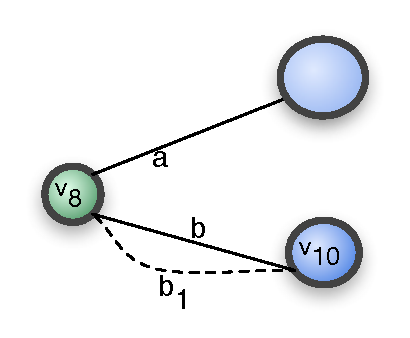
\includegraphics[width=0.35\textwidth]{social_news-gext-wv6}} 
	\subfloat[Forward]{\label{fig:groupext-weak}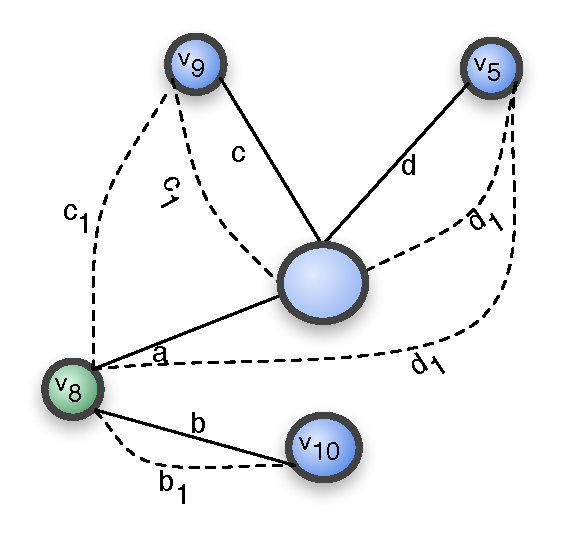
\includegraphics[width=0.35\textwidth]{social_news-gext-wfv6}}
	\caption{Group extension with $\nu_6$'s declination} 
	\label{fig:groupext-xv6}
\end{figure}

On the other hand, when a member accepts an invitation he can simply join the new group as a \emph{voter} or only on
condition that his own news are submitted to the group. Here, since $\nu_6$ has no news initially, he can only reply
``voting!". As well, when all the conditions are met for accepting the invitation $\nu_6$ should decide (provided the
deadline has not passed yet) whether he wants to extend the group further or simply move to a voting state.
Figure~\ref{fig:groupext-iv6} depicts the two scenarios when $\nu_6$ accepted the invitation.
\begin{figure} 
	\centering 
	\subfloat[Accept as voter]{
		\label{fig:groupext-accept}
		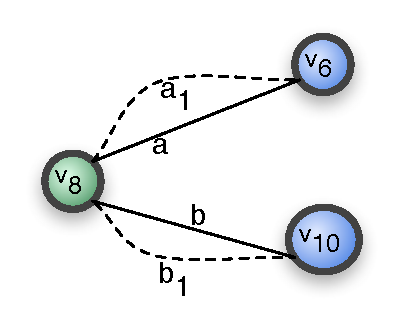
\includegraphics[width=0.35\textwidth]{social_news-gext-iv6}} 	
	\subfloat[Accept and extend]{
		\label{fig:groupext-accext}
		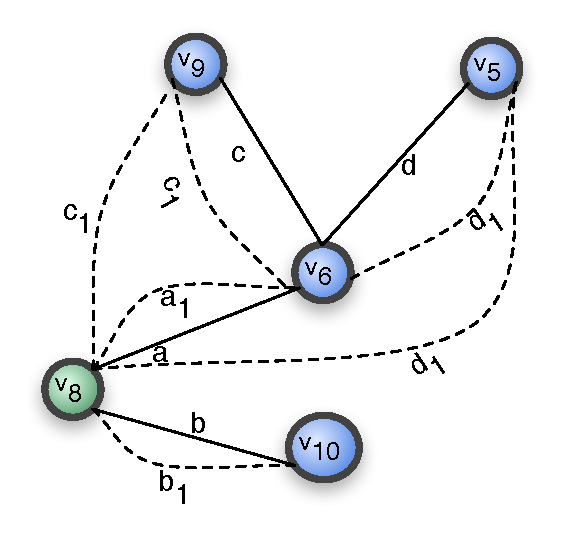
\includegraphics[width=0.35\textwidth]{social_news-gext-iextv6}} 
	\caption{Group extension with $\nu_6$'s acceptance}
	\label{fig:groupext-iv6}
\end{figure}
Equation~\ref{eq:pv6expr3} defines the process $P^{\nu_6}_{Acc}$, where $P^{\nu_6}_{Vote}$ represents the voting
behavior, while $P^{\nu_6}_{Ext}$ represents the extension behavior, which is similar to the forwarding behavior defined
in equations~\ref{eq:pv6expr2} and~\ref{eq:pv6expr22}. We define $P^{\nu_6}_{Vote}$ in section~\ref{sub:local_headline_adoption}. As
for $P^{\nu_6}_{Ext}$, we define it later in this section.

\begin{equation}
	\label{eq:pv6expr3}
	P^{\nu_6}_{Acc} \overset{df}{=}\overset{-}{a}^\prime<voting>.(P^{\nu_6}_{Vote} + P^{\nu_6}_{Ext}) 
\end{equation}

While extending the group $g^{\nu_8}$, $\nu_6$ should decide whether to send an invitation to both $\nu_5$ and $\nu_9$
or strictly one of them. Since, the decision to extend the headline has already been made, we do not consider any inactivity case in this choice. We define $P^{\nu_6}_{Ext}$ as follows.

\begin{equation}
	\label{eq:pv6expr4}
	\begin{gathered}
P^{\nu_6}_{Ext}\overset{df}{=}((\overset{-}{a}^\prime<c_1d_1>.(P^{\nu_6}_{For5}\mid P^{\nu_6}_{For9}))\mid P^{\nu_6}_{Vote} + (\overset{-}{a}^\prime<d_1>.P^{\nu_6}_{For5}\mid P^{\nu_6}_{Vote} +\\ \overset{-}{a}^\prime<c_1>.P^{\nu_6}_{For9}\mid P^{\nu_6}_{Vote}))
	\end{gathered}
\end{equation}

Another interesting scenario is the group formed by $\nu_2$. His immediate neighbors are $\nu_0$, $\nu_4$ and $\nu_3$. Let $g^{\nu_2}$ denote the group being extended and $P_{g^{\nu_2}}$ denote the process corresponding to the group extension. Finally, let $P^{\nu_2}$, $P^{\nu_0}$, $P^{\nu_4}$ and $P^{\nu_3}$ denote the individual processes corresponding to $\nu_2$, $\nu_0$, $\nu_4$ and $\nu_3$ respectively.

\begin{equation}
	\label{eq:gv2-formation}
	\boxed{P_{g^{\nu_2}}\overset{df}{=}(\nu G_2)(P^{\nu_2}\mid P^{\nu_0} \mid P^{\nu_4} \mid P^{\nu_3})}
\end{equation}

$P^{\nu_2}$ is very similar to $P^{\nu_8}$, $P^{\nu_0}$ and $P^{\nu_3}$ are similar to $P^{\nu_6}$ or $P^{\nu_{10}}$. The
node $\nu_4$ behaves slightly differently, since he has his own news $\nu_4^S$ to submit. Let $e$ denote the secret
channel created for communication between $\nu_2$ and $\nu_4$. When invited, $\nu_4$ will either decline or accept. The
declination process is similar to the usual case (reply ``no''). The acceptance process $P^{\nu_4}_{Acc}$ is defined
below as follows. The rest of the group extension is similar to what happened in $g^{\nu_8}$ extension.

\begin{equation}
	\label{eq:pv4expracc}
	P^{\nu_4}_{Acc} \overset{df}{=} \overset{-}{e}<\nu_4^S>.e(m).(\overset{-}{m}\mid (no.\mathbf{0} + yes.\tau))
\end{equation}

Using a formal approach to specify a system, whether concurrent or sequential, gives the advantage of verifying its
properties. For example, proposition~\ref{prop:gv8intercorrect} discusses the correct interactions which led to the
extension of the group $g^{\nu_8}$

\begin{proposition}
	\label{prop:gv8intercorrect}
	The extension of group $g^{\nu_8}$ is correct wrt the communication between its members. 
\end{proposition}

\begin{proof} We use reduction rules to prove the correctness of the group extension. Since we only provided a
complete specification for group $g^{\nu_8}$'s extension it is easier to verify the correctness of the interactions
during that group extension, the process $P_{g^{\nu_8}}$. Starting from the parallel composition in
equation~\ref{eq:gv8-formation}, we verify that all the processes reduce to their voting state or inactivity for those
which declined the invitation. Here, we focus on the case where $\nu_8$ only invites $\nu_6$. The other cases are similar.

\[
\begin{array}{l}
	(\ref{eq:gv8-formation})\rightarrow \mathbf{0} + (\nu a_1:G_8[\mathbf{C}_{\nu_6^8}], \nu b_1:G_8[\mathbf{C}_{\nu_{10}^8}])(P^{\prime\nu_8} + (P^{\prime\prime\nu_8} + P^{\prime\prime\prime\nu_8}))\\
	\mid (\nu a^\prime:G_8[\mathbf{C}_{\nu_6^8}]) (a(a^\prime).a^\prime(m).P^{\nu_6}_\propto)\mid (P^{\nu_{10}})
\end{array}
\]

For the sake of succinctness we omit the instances of the secret channels created to support communication between
processes. The reduction above reveals an internal choice, which requires to study several cases. First, in case of
inactivity, no interaction occurs since $\nu_8$ sends no message out. The second case corresponds to when $\nu_8$ decides
to involve both $\nu_6$ and $\nu_{10}$. The two remaining cases are when $\nu_8$ involves strictly one of his neighbors.
We refine the reduction as indicated below. In the following we use \emph{COM}, the communication rule (a read and a
write).

\[
\begin{array}{l} 
	(\ref{eq:gv8-formation})\rightarrow  \overset{-}{a}<a_1>.\overset{-}{a}_1<\nu_8^S>.P^{\nu_8}_{\propto a_1R} \mid a(a^\prime).a^\prime(m).P^{\nu_6}_\propto\\
	(\ref{eq:gv8-formation})\xrightarrow{COM} \overset{-}{a}_1<\nu_8^S>.P^{\nu_8}_{\propto a_1R} \mid [^{a^\prime}/_{a_1}]a_1(m).P^{\nu_6}_\propto\\
	(\ref{eq:gv8-formation})\xrightarrow{COM} P^{\nu_8}_{\propto a_1R} \mid [^{a^\prime}/_{a_1}, ^m/_{\nu_8^S}]P^{\nu_6}_\propto\\
	(\ref{eq:gv8-formation})\xrightarrow{} ((a_1(m^\lambda).(\overset{-}{m}^\lambda\mid (no.\tau.P^{\nu_8}_{\propto a_1} + forward.a_1(\hat{g})\mid !P^{\nu_8}_{\propto R} + voting.\tau.P^{\nu_8}_{\propto a_1}\\  + \hat{g}.!P^{\nu_8}_{\propto R}  + \nu_\imath^S.(\overset{-}{a}_1<no> + \overset{-}{a}_1<yes>.\tau^\prime).P^{\nu_8}_{\propto a_1})))) \mid [^{a^\prime}/_{a_1}, ^m/_{\nu_8^S}] (P^{\nu_6}_{Dec} + P^{\nu_6}_{Acc})\\
\end{array} 
\]

From this point we now have two alternatives: $\xrightarrow{+Dec}$ where we continue the reduction assuming
$P^{\nu_6}_{Dec}$ has been selected and $\xrightarrow{+Acc}$, which continues the reduction assuming $P^{\nu_6}_{Acc}$
has been selected.

\[
\begin{array}{l}
	(\ref{eq:gv8-formation})\xrightarrow{+Dec} ((a_1(m^\lambda).(\overset{-}{m}^\lambda\mid (no.\tau.P^{\nu_8}_{\propto a_1} + \hat{g}.!P^{\nu_8}_{\propto R} + forward.a_1(\hat{g})\mid !P^{\nu_8}_{\propto R} + voting.\tau.P^{\nu_8}_{\propto a_1}\\ + \nu_\imath^S.(\overset{-}{a}_1<no> + \overset{-}{a}_1<yes>.\tau^\prime).P^{\nu_8}_{\propto a_1})))) \mid [^{a^\prime}/_{a_1}, ^m/_{\nu_8^S}] (\overset{-}{a}_1<no>.0 +\\ \overset{-}{a}_1<forward>(\overset{-}{a}_1<c_1d_1>.(P^{\nu_6}_{For5}\mid P^{\nu_6}_{For9}) + (\overset{-}{a}_1<d_1>.P^{\nu_6}_{For5} + \overset{-}{a}_1<c_1>.P^{\nu_6}_{For9})))\\
\end{array}
\]

At this point we have non determinism on both sides. If $\nu_6$ decides not to forward the invitation to any of his
neighbors, there will be inactivity on the righthand side of the parallel composition, which ends the interaction between
both nodes. Note that $\nu_8$ continues listening to other invited members or prepares to notify that the deadline has
passed.

\[
\begin{array}{l}
	(\ref{eq:gv8-formation})\xrightarrow{COM} P^{\nu_8}_{\propto a_1} \mid [^{a^\prime}/_{a_1}, ^m/_{\nu_8^S}] 0
\end{array}
\]

On the other hand let us consider that $\nu_6$ forwards the invitation to his neighbors. As it appears, the interaction will end between $\nu_6$ and $\nu_8$ and continue with the other members ($\nu_5$ and $\nu_9$).

\[
\begin{array}{l}
	(\ref{eq:gv8-formation})\xrightarrow{COM} [^{\hat{g}}/_{<c_1d_1>}](!P^{\nu_8}_{\propto R})\mid [^{a^\prime}/_{a_1}, ^m/_{\nu_8^S}] (P^{\nu_6}_{For5}\mid P^{\nu_6}_{For9})\\
	(\ref{eq:gv8-formation})\xrightarrow{COM} [^{\hat{g}}/_{<c_1d_1>}]!P^{\nu_8}_{\propto R}\mid [^{a^\prime}/_{a_1}, ^m/_{\nu_8^S}] ((\overset{-}{d}<d_1>.\overset{-}{d}_1<\nu_8^S>)\mid P^{\nu_5})\mid\\ (\overset{-}{c}<c_1>.\overset{-}{c}_1<\nu_8^S>)\mid P^{\nu_9})\\
\end{array}
\]

By definition, the processes $P^{\nu_5}$ and $P^{\nu_9}$ are similar to the processes $P^{\nu_6}$ and $P^{\nu_{10}}$. The
messages sent out by $\nu_6$ will be read by $\nu_5$ and $\nu_9$, who in turn will reply to $\nu_8$ (process $P^{\nu_8}_{\propto R}$).

In case of the $\xrightarrow{+Acc}$ alternative, we have the following reductions.

\[
\begin{array}{l}
	(\ref{eq:gv8-formation})\xrightarrow{+Acc} ((a_1(m^\lambda).(\overset{-}{m}^\lambda\mid (no.\tau.P^{\nu_8}_{\propto a_1} + \hat{g}.!P^{\nu_8}_{\propto R} + forward.a_1(\hat{g})\mid !P^{\nu_8}_{\propto R} + voting.\tau.P^{\nu_8}_{\propto a_1}\\ + \nu_\imath^S.(\overset{-}{a}_1<no> + \overset{-}{a}_1<yes>.\tau^\prime).P^{\nu_8}_{\propto a_1})))) \mid [^{a^\prime}/_{a_1}, ^m/_{\nu_8^S}] \overset{-}{a}_1<voting>.(P^{\nu_6}_{Vote} + P^{\nu_6}_{Ext})\\
	(\ref{eq:gv8-formation})\xrightarrow{COM} \tau.P^{\nu_8}_{\propto a_1} \mid [^{a^\prime}/_{a_1}, ^m/_{\nu_8^S}] (P^{\nu_6}_{Vote} + P^{\nu_6}_{Ext})\\	
	(\ref{eq:gv8-formation})\xrightarrow{\tau} P^{\nu_8}_{\propto a_1} \mid [^{a^\prime}/_{a_1}, ^m/_{\nu_8^S}] (P^{\nu_6}_{Vote} + P^{\nu_6}_{Ext})\\	
\end{array}
\]

If $\nu_6$ chooses not to forward the invitation to any of his neighbors, he will move to the voting state
($P^{\nu_6}_{Vote}$). On the other hand, if he chooses to forward to any of his neighbors, the process is similar to what
happened in forward case with declination. In summary, we sketched the proof that the interaction between members in
order to extend a group is correct, i.e., the group extension will end up with processes in a voting state or inactivity.
The proof for the other cases is quite similar to the one we discussed here. Thus, we omit them here.
\end{proof}

% subsection group_extension (end)

\subsection{Local Headline Adoption} % (fold)
\label{sub:local_headline_adoption}

From the scenario we discussed in section~\ref{sub:group_extension}, we obtained two groups: $g^{\nu_8}$ and $g^{\nu_2}$. The
group $g^{\nu_8}$ involves $\nu_8$ (the initiator of the group), $\nu_6$, $\nu_{10}$, $\nu_{11}$, $\nu_9$ and
$\nu_5$. It has only one set of news, submitted by $\nu_8$, $\nu_8^S=<\alpha_0^8, \ldots,\alpha_k^8>$. The second group,
$g^{\nu_2}$, involves $\nu_2$ (as initiator) and $\nu_0$, $\nu_1$, $\nu_4$ and $\nu_3$. It has two sets of news
$<<\alpha_0^2, \ldots,\alpha_\ell^2>,<\alpha_0^4, \ldots,\alpha_m^4>>$ originating from $\nu_2$ and $\nu_4$.
Figure~\ref{fig:groups} depicts the two groups formed at the end of the group extension stage.
\begin{figure}
	\centering 
	\subfloat[$g^{\nu_2}$ group]{\label{fig:groupext-gv2}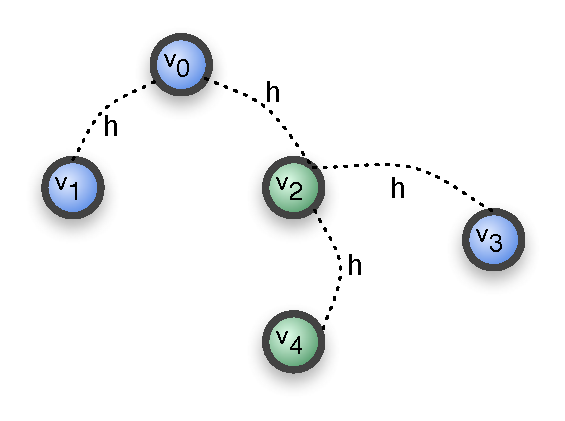
\includegraphics[width=0.35\textwidth]{social_news-gv2-aformation}} 
	\subfloat[$g^{\nu_8}$group]{\label{fig:groupext-gv8}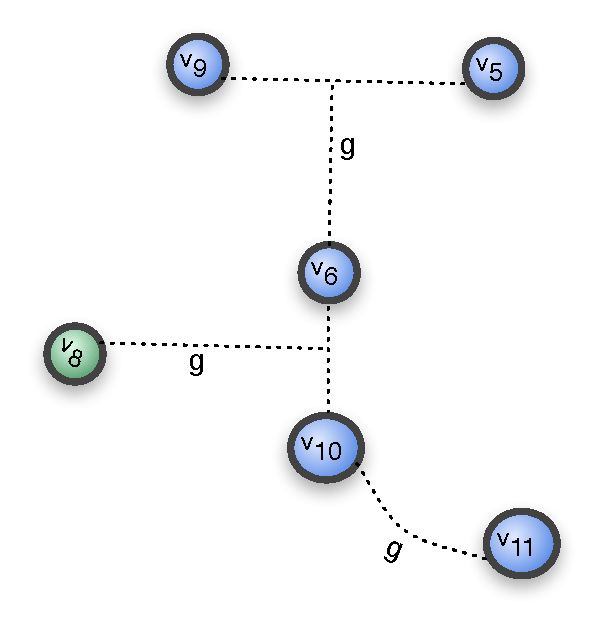
\includegraphics[width=0.35\textwidth]{social_news-gv8-aformation}}
	\caption{$g^{\nu_8}$ and $g^{\nu_2}$ groups} 
	\label{fig:groups}
\end{figure}

When the voting exercise completes, each group gets its set of local headlines. Let $<\alpha_0^{g^{\nu_2}}, \ldots,
\alpha_p^{g^{\nu_2}}>$ denote the local headline set for $g^{\nu_2}$, while $<\alpha_0^{g^{\nu_8}}, \ldots,
\alpha_q^{g^{\nu_8}}>$ denote the one for $g^{\nu_8}$. In this paper, we do not enter any detail about the voting
procedure itself. Algorithms to support automated voting procedures have been discussed at length, in \emph{Social Choice
theory}, a discipline overlapping \emph{game theory} and \emph{Computer Science}. For example, several voting algorithms
have been discussed by Brams and Fishburn in~\cite{Brams-Fishburn:04}. We simply assume that members of a newly extended
group will agree on a voting procedure and will abide by it.

In this paper, we only emphasize the interactions during the voting procedure. We define both the behavior of those
members who submitted news to the group as well as that of simple voters. In group $g^{\nu_8}$, all the members
will vote except for $\nu_8$, the only member who submitted news. However, $\nu_8$ can be employed as an observer for the
voting exercise. We do not risk a conflict of interest here since all the members use the same channel to submit their
votes, i.e., \emph{transparency}. As an observer, $\nu_8$ has first to read the votes as they are sent by the voters,
then process the votes and proclaim the results. We consider that $P^{\nu_8}_{Vote}\overset{df}{=}P_{g^{\nu_8}}^{Ob}$. We
define the process $P_{g^{\nu_8}}^{Ob}$ in equation~\ref{eq:voteobs}.

\begin{equation}
	\label{eq:voteobs}
	P_{g^{\nu_8}}^{Ob}\overset{df}{=}!(h(\ldots(\omega_\theta, \alpha_\imath)\ldots(\omega_{\theta^\prime}, \alpha_\jmath)\ldots)).\tau.\overset{-}{g}<\alpha_0^{g^{\nu_8}}, \ldots,
	\alpha_q^{g^{\nu_8}}> (\theta, \theta^\prime = 1,\ldots, 5)
\end{equation}

A voter first reads the voting channel, then takes a silent transition to decide which news to vote for as local headline
and finally communicates his vote through the common channel. For example,  $P^{\nu_6}_{Vote}$ is defined as follows.
\begin{equation}
	\label{eq:v6voting}
	P^{\nu_6}_{Vote}\overset{df}{=}a_1(g).\tau.\overset{-}{g}<\ldots(\omega_\theta, \alpha_\imath)\ldots(\omega_{\theta^\prime}, \alpha_\jmath)\ldots(\omega_{\theta^{\prime\prime}}, \alpha_\ell)\ldots>
\end{equation}

\begin{proposition}
	\label{prop:gv8votecorrect}
	The voting process in group $g^{\nu_8}$ is consistent. 
\end{proposition}

\begin{proof}
 As a follow-up to the proof to proposition~\ref{prop:gv8intercorrect} in section~\ref{sub:group_extension}, we obtain a
parallel composition of the members who did not go into inactivity. The only new element is the observer behavior which
replaced $\nu_8$'s voting behavior. Because of the replication of the \emph{read} prefix in the observer
($P_{g^{\nu_8}}^{Ob}$), any message sent by a voter is well captured and considered later in the vote processing.
Besides, the internal actions are silent transitions. As such, they do not require any interaction with other processes.
\end{proof}

In the second group ($g^{\nu_2}$) a few interesting points are worth a mention. By virtue of being news submitters both
$\nu_2$ and $\nu_4$ are de facto candidates for the observer role. However, observing a voting procedure in this
application is quite straightforward. Therefore, it does not require to mobilize two members for the observer role. Note
that there are several possibilities. There could be an election phase to decide which of $\nu_4$ and $\nu_2$ should be
allowed to observe the voting exercise. There could be some negotiation between the two members, and hopefully a
consensus will be reached. Here, we choose a simpler solution. Node $\nu_2$, as the initiator of the group extension, is
systematically in charge of observing the voting exercise, thus forcing $\nu_4$ to inactivity.

% subsection local_headline_adoption (end)

\subsection{Generalization} % (fold)
\label{sub:generalization}

All through section~\ref{sec:group_extension_local_headline}, we used examples to specify the behaviors of members of the social network
involved in the identification of local headlines. In this section we wish to generalize the specifications of these processes. This generalization covers both the group extension and the voting procedure.

Let $\nu_\imath$ denote a node wishing to submit news to {\tt Social News}. Let $P^{\nu_\imath}$ denote the process representing his behavior. Let $\nu_{\jmath 0}$, \ldots, $\nu_{\jmath\ell}$ denote his immediate neighbors. Let $P^{\nu_{\jmath 0}}$, \ldots, $P^{\nu_{\jmath \ell}}$ denote the processes corresponding to their behaviors, respectively. As well, let $a_{\jmath 0}$, \ldots, $a_{\jmath\ell}$ denote the links between $\nu_\imath$ and each of the immediate neighbors.

A group extension initiated by $\nu_\imath$ (denoted by $P_{g^{\nu_\imath}}$) is represented as follows, where
$P^{\nu_{\jmath u}}$ corresponds to any of the processes representing $\nu_\imath$'s immediate neighbors. Here we use the
replication operator, $!$, since it is \emph{equivalent} to a parallel composition of as many of these processes as
required.

\begin{equation}
	\label{eq:gvi-formation}
	P_{g^{\nu_\imath}}\overset{df}{=}(\nu G_\imath)(P^{\nu_\imath}\mid !P^{\nu_{\jmath u}})	\mbox{ with } u=0,\ldots,\ell
\end{equation}

$P^{\nu_\imath}$ is a non deterministic choice between inactivity and any process involving all or a subset of the
neighbors. For each type of process that can be selected, a particular instance of $G_\imath$ needs to be created. Let
$a^\prime_{\jmath\ell}$ denote a new instance of $G_\imath$ created to interact with $\nu_{\jmath\ell}$. We define
$P^{\nu_\imath}$ as follows.

\begin{equation} 
	\label{eq:pviexpr1}
	\begin{gathered} 
		P^{\nu_\imath} \overset{df}{=} \mathbf{0} + ((\nu a^\prime_{\jmath 0}:G_\imath[\mathbf{C}_{\nu^\imath_{\jmath 0}}], \ldots, \nu a^\prime_{\jmath\ell}:G_\imath[\mathbf{C}_{\nu^\imath_{\jmath\ell}}]) P^{\prime\nu_\imath} + \ldots + P^{m\nu_\imath} + \ldots + P^{k\nu_\imath})
	\end{gathered}
\end{equation}

Generally a process $P^{m\nu_\imath}$ is a parallel composition of processes $P^{t\nu_\imath}$.

\begin{equation} 
	\label{eq:pviexpr11}
	\begin{gathered} 
		P^{m\nu_\imath}\overset{df}{=}!P^{t\nu_\imath}\\
		P^{t\nu_\imath}\overset{df}{=}\overset{-}{a}_{\jmath t}<a^\prime_{\jmath t}>.\overset{-}{a}^\prime_{\jmath t}<\nu^S_\imath>.P^{t\nu_\imath}_{\propto a^\prime_{\jmath tR}}\\
		P^{t\nu_\imath}_{\propto a^\prime_{\jmath t}R}\overset{df}{=}((a^\prime_{\jmath k}(m^\delta).(\overset{-}{m}^\delta\mid (no.\tau.P^{\nu_\imath}_{\propto a^\prime_{\jmath t}} + \hat{h}.!P^{\nu_\imath}_{\propto R} + forward.a^\prime_{\jmath t}(\hat{h})\mid !P^{\nu_\imath}_{\propto R} +\\ voting.\tau.P^{\nu_\imath}_{\propto a^\prime_{\jmath t}} + \nu_\imath^S.(\overset{-}{a}^\prime_{\jmath t}<no> + \overset{-}{a}^\prime_{\jmath t}<yes>.\tau).P^{\nu_\imath}_{\propto a^\prime_{\jmath t}}))))\\
		P^{\nu_\imath}_{\propto R}\overset{df}{=}((u(m^{\delta\prime}).(\overset{-}{m}^{\delta\prime}\mid (no.\tau + \hat{h}^\prime.!P^{\nu_\imath}_{\propto R} + forward.u(\hat{h})\mid !P^{\nu_\imath}_{\propto R} +\\ voting.\tau + \nu_\imath^S.(\overset{-}{u}<no> + \overset{-}{u}<yes>.\tau)))))\\ (\mbox{ with } u\in\bigcup\hat{h}, \mbox{ union of the names communicated to } \nu_\imath)
	\end{gathered}
\end{equation}

The process $P^{\nu_\imath}_{\propto a^\prime_{\jmath t}}$ is a non deterministic choice between the time-up process ($P^{\nu_\imath}_{TimeUp}$) and the reading process $P^{t\nu_\imath}_{\propto a^\prime_{\jmath t}R}$.

\begin{equation} 
	\label{eq:pviexpr12}
	\begin{gathered} 
		P^{t\nu_\imath}_{\propto a^\prime_{\jmath t}}\overset{df}{=}(P^{t\nu_\imath}_{TimeUp} + P^{t\nu_\imath}_{\propto a^\prime_{\jmath t}R})\\
		P^{t\nu_\imath}_{TimeUp}\overset{df}{=}(\nu g_\imath:G_\imath[\mathbf{C}_{\nu^\imath}])\overset{-}{s}<g_\imath>.(\tau.\mathbf{0} + P^{\nu_\imath}_{Vote}) (\mbox{ with } s\in \hat{C}_{\nu_\imath})	
	\end{gathered}
\end{equation}

On the other hand any of the invited members to the group extension behaves as follows.

\begin{equation} 
	\label{eq:pvjexpr11}
	\begin{gathered}
		P^{\nu_{\jmath u}}\overset{df}{=} (\nu b_{\jmath u}:G_\imath[\mathbf{C}_{\nu^\imath}, \mathbf{C}_{\nu_{\jmath u}^\imath}]) (a_{\jmath u}(b_{\jmath u}).b_{\jmath u}(m^{\jmath u}).P^{\nu_{\jmath u}}_\propto)\\
		P^{\nu_{\jmath u}}_\propto \overset{df}{=} (P^{\nu_{\jmath u}}_{Dec} + P^{\nu_{\jmath u}}_{Acc})		
	\end{gathered}
\end{equation}

\begin{equation} 
	\label{eq:pvjexpr12}
	\begin{gathered}
		P^{\nu_{\jmath u}}_{Dec}\overset{df}{=}\overset{-}{b}_{\jmath u}<no> + \overset{-}{b}_{\jmath u}<forward>.\overset{-}{b}_{\jmath u}<\hat{h}^\prime>\mid !P^{\nu_{\jmath u}}_{For}\\
		P^{\nu_{\jmath u}}_{For}\overset{df}{=}\overset{-}{b}_{\jmath um}<b^\prime_{\jmath um}>.\overset{-}{b}^\prime_{\jmath um}<\nu^S_\imath>\mid P^{\nu_{\jmath um}}
	\end{gathered}
\end{equation}

\begin{equation} 
	\label{eq:pvjexpr13}
	\begin{gathered}
		P^{\nu_{\jmath u}}_{Acc}\overset{df}{=}(\overset{-}{b}_{\jmath u}<voting>.(P^{\nu_{\jmath u}}_{Vote} + P^{\nu_{\jmath u}}_{Ext})) + (\overset{-}{b}_{\jmath u}<\nu_{\jmath u}^S>.\\{b}_{\jmath u}(m^\lambda).(\overset{-}{m}^\lambda\mid no.\tau + yes.(\tau + !P^{\nu_{\jmath u}}_{For}))\\
		P^{\nu_{\jmath u}}_{Ext} \overset{df}{=}(\ldots +  P^{w\nu_{\jmath u}}_{Ext} + \ldots)\\
		P^{w\nu_{\jmath u}}_{Ext}\overset{df}{=}\overset{-}{b}_{\jmath u}<\hat{h}^\prime>\mid !P^{\nu_{\jmath u}}_{For}\mid P^{\nu_{\jmath u}}_{Vote}\\
	\end{gathered}
\end{equation}


Finally, we define the voting processes as follows.

\begin{equation} 
	\label{eq:pvivote11}
	\begin{gathered}
		P^{\nu_\imath}_{Vote}\overset{df}{=}P_{g^{\nu_\imath}}^{Ob}\\
		P^{\nu_{\jmath u}}_{Vote}\overset{df}{=}b_{\jmath u}(g^\imath).\tau.\overset{-}{g}^\imath<\ldots(\omega_\theta, \alpha_\imath)\ldots(\omega_{\theta^\prime}, \alpha_\jmath)\ldots>\\
		P_{g^{\nu_\imath}}^{Ob}\overset{df}{=}!(h(\ldots(\omega_\theta, \alpha_\imath)\ldots(\omega_{\jmath^\prime}, \alpha_\jmath)\ldots)).\tau.\overset{-}{g}^\imath<\alpha_0^{g^{\nu_\imath}}, \ldots,
		\alpha_q^{g^{\nu_\imath}}>
	\end{gathered}
\end{equation}

\begin{proposition}
	\label{prop:genercor}
	Globally, the local headline adoption  step is correct.
\end{proposition}

\begin{proof}
	The proof of this proposition follows from the generalization of propositions~\ref{prop:gv8intercorrect} and~\ref{prop:gv8votecorrect}.
\end{proof}

% subsection generalization (end)

% section group_extension_&_local_headline (end)